\documentclass[a4paper,10pt]{article}
\usepackage{a4wide}
\usepackage[final]{graphicx}
\usepackage{epstopdf}
\usepackage[english]{babel}
\usepackage[small,bf]{caption}
\usepackage{subcaption}
\usepackage{graphicx,latexsym,subfig,amsmath,amssymb,amsthm,listings,pdfpages,epstopdf,alltt,enumerate}
\pagestyle{myheadings}

%%%%%%%%%%%%%%%%%%%%%%%%%%%%%%%%%%%%%%%%%%%%%%%
\newcommand{\Title}{Monte Carlo Simulation of Polymers}
\newcommand{\Author}{J. Moeskops, L. Janssen}
\newcommand{\Date}{\today}
\newcommand{\Subject}{2nd assignment of ICCP}
\newcommand{\Mail}{jonnemoeskops@hotmail.com, laurensjanssen92@gmail.com}
%%%%%%%%%%%%%%%%%%%%%%%%%%%%%%%%%%%%%%%%%%%%%%%

\begin{document}

%%%%%%%%%%%%%%%%%%%%%%%%%%%%%%%%%%%%%%%%%%%%%%%
%%%  Begin Header
\markright{\footnotesize\textnormal{\textbf{\Title}}~~~\Author}
\thispagestyle{plain} \noindent\begin{center}
Delft University of Technology - Applied Physics - ICCP
\par\bigskip
\end{center}
\par\begin{center}
{\LARGE\textbf{\Title}}\par\bigskip{\large \Author}
\end{center}
\par\bigskip
\begin{center}{\small
\begin{tabular}{ll}\hline
\textbf{Date:}& \Date\\
\textbf{Course:}& AP3081TU D - International Masters Course on Computational Physics\\
\textbf{Subject:}& \Subject\\
\textbf{Students:} & J. Moeskops (4023250), L. Janssen (4117239) \\
\textbf{E-mail:} & \Mail\\\hline
\end{tabular}}
\end{center}
\par\bigskip
%%%  End Header
%%%%%%%%%%%%%%%%%%%%%%%%%%%%%%%%%%%%%%%%%%%%%%%

\begin{figure}[ht!]
\centering
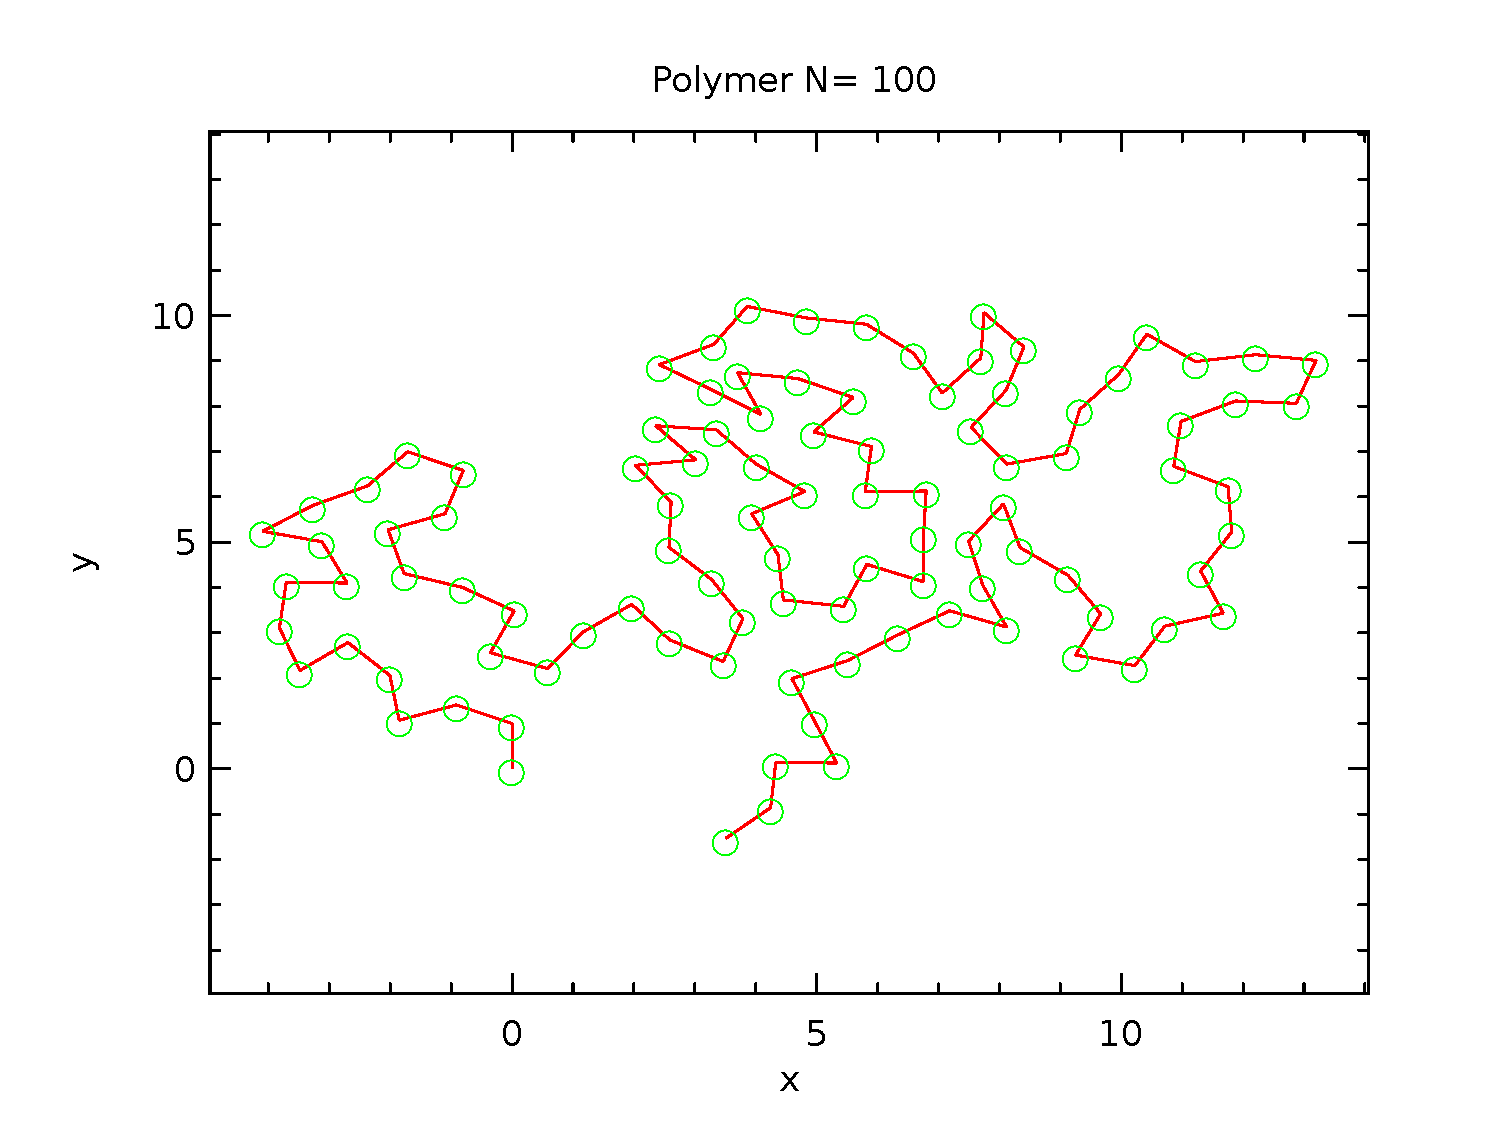
\includegraphics[width=1.0\textwidth]{voorblad.pdf}
\label{fig:voorblad}
\end{figure}
\pagebreak



\begin{abstract}
In this report the simulation and results of a dilute polymer solution is described.  A Monte Carlo simulation in 2D-space is performed to grow polymers segment by segment. The segments only interact with each other through the Lennard-Jones Potential. A Rosenbluth like algorithm is applied to add new segments, favouring lowest energy configurations. To achieve more reliable results a Pruning and Enrichments technique is applied, which promotes lower energy configurations and kills higher energy configurations. The simulation is used to calculate polymer properties in 2D like End-to-end distance and Gyradius. A total of 10000 polymers are grown to a length of 350 segments.
\end{abstract}

\section*{Introduction}
The study of polymers is important for its wide uses in industry and everyday life. Polymers are composed of an integer number of unit-segments, or monomers, which together form a polymer. When ensembling a polymer by repeating unit segments it can take all sorts of configurations, depending on the angle between subsequent segments. This angle is determined under the influence of the solvent of the polymer and interaction forces between the molecules. 

Such a polymer can be modelled by representing each segment as a ``bead'' which has a fixed distance to the previous bead. Depending on the polymer and the solvent a force, which acts between the beads, can be introduced. In this research a dilute polymer solution in 2D is simulated and the force between beads is modelled as a Lennard-Jones force.

A common method used for simulating polymers like this is the Rosenbluth algorithm, which adds subsequent beads trying to avoid high energy configurations. In this research we will make use of a Rosenbluth like algorithm which makes additional use of a pruning and enrichment strategy to build polymers. This strategy promotes low energy configurations and kills high energy configurations. 

Interesting properties, which are studied, are the average End-to-end distance as a function of length and how compact the polymer becomes as a function of length, this can be expressed in terms of the radius of gyration, or Gyradius.  

\section*{Model}
In a dilute polymer solution we can study the effect of a solvent by looking at ensembles of individual polymers. A good solvent means that the free energy of a polymer segment that is surrounded by solvent will be less than that of a segment which is close to other segments in the polymer. By introducing an effective repulsion between polymer segments we achieve the same effect.

The model aimed for is one that preserves the important properties of a polymer without incorporating all the atomic details of its structure. Polymers are large molecules in which a number of repeated segments form long chains. The number of such segments $N$ is typically $10^3 - 10^5$. In this report we will be working on the large scale of the polymer and we will therefore make the simplification of universal behaviour. This means that the properties of the polymer are not dependent on the chemical nature of it and we can look at the segments as closed units or ``beads''. Neighbouring beads have a fixed mutual distance and no further interaction. Furthermore, the beads repel when they overlap and experience an attractive van der Waals' interaction on longer distances. One last interaction is the effective repulsion between segments due to the solvent effect, described earlier. The interaction of non-neighbouring beads can therefore be described by a Lennard-Jones interaction. Because the beads repel each other the polymer represents a self-avoiding walk or SAW -- as opposed to the random walk.

The polymers in this report are studied in an off-lattice model in two dimensions. In the next sections this model is implemented in an algorithm.

\section*{Algorithm}
\subsection*{Rosenbluth Algorithm}
		• initial configuration
		• adding beads (weights, angles, ...)
		• total weight factor of a polymor (because the Rosenbluth algorithm has bias towards dense configurations, which is a trade-off of solving atrition)

The most basic method to simulate a SAW is that of simple sampling which goes as follows: place a first segment at the origin and a second one at unit distance. Choose a random angle to place the next segment at unit distance from the previous segment and check the self-avoidance. If the chain is self-avoiding, the growth process continues until the desired length is reached. If not, the polymer is discarded and we start again from scratch. The completed SAW's are independent of each other and occur with the same probability but this probability gets exponentially small for increasing length $N$. This problem of very low efficiency is called the attrition problem.

The Rosenbluth algorithm (also called RR) aims to solve this attrition problem by not putting the next bead in the chain at random but by scanning the environment for neighbouring beads and only choosing those directions which lead to self-avoidance. It is clear that the attrition is strongly reduced but also a bias is introduced. A SAW is no longer produced with uniform probability, but with probability inversly proportional to the number of open directions:

\begin{equation} \label{eq:prob_RR}
	P\left(\vec{x}\right) = \prod_{i=1}^{N} \frac{1}{n_i} .
\end{equation}

Here $n_i$ is the number of open directions for adding bead number $i$ and $\vec{x}$ is the position vector of all the beads in the polymer.

Polymers that have a smaller $n_i$ have thus a higher probability of being generated and this method therefore has a bias towards dense configurations. This bias can be corrected for by incorporating the weight $W\left( \vec{x} \right) \propto 1/ P\left( \vec{x} \right)$ when calculating observables.

The bias towards dense configurations also means that the RR method is not usefull for long SAW's. Only a small number of polymers generated by the RR method will have large end-to-end distance (and large weight). This portion of large polymers becomes smaller with increased number of beads $N$. The RR method has to be repeated a great number of times to sample long SAW's and is therefore not suitable. The broad distribution of weights leads to a large variance of the calculated observables.

\subsection*{Pruning and Enriching (PERM)}
A more modern algorithm is the Pruned-Enriched Rosenbluth Method or PERM. The main idea of PERM is to keep the distribution of weights within certain bounds by killing polymers with a small weight and cloning polymers with a large weight.

Suppose that a polymer chain is created up to bead number $i$ using the RR method and has a weight $W_i$. In order to prevent this $W_i$ from fluctuating the sample should be either "pruned" or "enriched" when this weight becomes too small or too large respectively. This is done in the following way:

\begin{itemize}
  \item If $W_i$ becomes too small (i.e. $W_i < \textup{LowLim}$) the polymer is destroyed with a probability of 50\%. If the polymer is not destroyed, its weight is doubled and the growth continues.
  \item If $W_i$ becomes too large (i.e. $W_i > \textup{UpLim}$) the polymer is cloned and its weight is halved. The growth now continues for both polymers.
\end{itemize}

\subsection*{PERM and dilute polymer solution}

\section*{Simulation and Results}
\subsection*{Simulation}
In the simulation 10000 polymers were grown for the RR method and 5000 polymers were grown for the algorithm including PERM. Each polymer bead has a reduced fixed length of 1.0 with respect to the previous bead. The acting Lennard-Jones potential uses reduced units of $\epsilon=0.25$ and $\sigma=0.8$, also the reduced temperature is set to $T=1.0$. All the polymers are grown to a length of $N=350$. 

We are interested in the average End-to-end-distance $R$ as a function of polymer length $N$ and in the average Gyradius as a function of length $N$. The average End-to-end-distance $R$ will be compared to the theoretical result, according to which it should relate to $N$ as $R\propto N^{3/4}$.

In order to leave out polymers which have become trapped and are therefore forced to cross themselves, we apply pruning and enriching. The limits for pruning and enriching are determined and dynamically updated according to the average weight of each polymer for each length $N$. Values of $\alpha_-=1.2$ and $\alpha_+=2.0$ are used. This method ensures only polymers which haven't trapped themselves are considered in the results. A comparison is made of the results with PERM and without.
\subsection*{Results}
\subsubsection*{Average End-to-end distance $R$}

In Figure \ref{fig:etoe_rr} and \ref{fig:etoe_perm} the square of the average End-to-end distance $R^2$ is plotted on a log-log scale. It is seen that the results for $N>100$ are a lot better if the PERM algorithm is used. Just as expected and explained earlier, the variance for large polymers becomes bigger when using the standard Rosenbluth algorithm, which is why there is a noticable deviation from the theoretical fit for $N>100$. In the case of the PERM algorithm, the population size is also plotted and remains fairly constant, especially for lengths below $N \approx 100$.

\begin{figure}[ht!]
\centering
\includegraphics[width=0.8\textwidth]{figures/N350_I10000_E2E_RR3}
\caption{Square of the End-to-end distance $R^2$ as a function of polymer length $N$, the red dotted line is the theoretical fit of $R^2=a\cdot \left(N-1\right)^{3/2}$ to the first 100 data points, where $a$ was found to be $0.86$. 10000 polymers are grown with Rosenbluth algorithm.}
\label{fig:etoe_rr}
\end{figure}

\begin{figure}[ht!]
\centering
\includegraphics[width=0.8\textwidth]{figures/N350_E2E_PERM3}
\caption{Square of the End-to-end distance $R^2$ as a function of polymer length $N$, the red dotted line is the theoretical fit of $R^2=a\cdot \left(N-1\right)^{3/2}$ to the first 250 data points, the population sizes for each length $N$ are given as well. Polymers are grown with PERM algorithm. The fit constant $a$ was found to be $0.77$.}
\label{fig:etoe_perm}
\end{figure}

\subsubsection*{Average Gyradius $G$}

Radius of gyration or gyradius is a measure of the size of a configuration. Is is the root mean square distance of the beads in a configuration to the centre of mass. The gyradius is thus calculated as:

\begin{equation}
    G^2 = \frac{1}{N} \sum_{i=1}^N \left( \mathbf{x_i} - \mathbf{x_{mean}} \right)^2
\end{equation}
with $\mathbf{x_{mean}}$ the mean position of the beads, which is the same as the centre of mass since all beads have identical mass. One reason that the radius of gyration is an interesting property is that it can be determined experimentally with static light scattering as well as with small angle neutron- and x-ray scattering. This allows theoretical polymer physicists to check their models against reality.\cite{grosberg1994}

In Figure \ref{fig:gyradius} the average Gyaradius $G$ is plotted on a linear scale. The data used is that of the same PERM simulation as in figure \ref{fig:etoe_perm}.

\begin{figure}[ht!]
\centering
\includegraphics[width=0.8\textwidth]{figures/N350_Gyradius_PERM3}
\caption{Gyradius $G$ as a function of polymer length $N$.}
\label{fig:gyradius}
\end{figure}

\section*{Conclusion}
In this report two algorithms were discussed for Monte Carlo simulations of 2D polymers. The first algorithm is based on Rosenbluth's method of adding one bead after another, while favouring low energy confirmations and implementing a self avoiding interaction. It was found that the pruning and enriching significantly decreased the variance of the calculated observables and made is possible to produce polymers of up to 350 beads long.

\end{document}
